\chapter{Overview of the Full-Stack Design}%
\label{s_architecture}

The system comprises four logical functions that together implement the proposed framework:
(i) a WebServer that provides authoritative aeronautical topology (vertiports and the air-corridor network),
(ii) a Planner that computes candidate 4D trajectories over that topology and performs iterative conflict checks,
(iii) an internal conflict-checking module embedded within the Planner that screens candidate routes against active traffic,
and (iv) a U-space Service Provider (USSP) that validates, authorizes, and supervises the flight-plan lifecycle.

Figure \ref{fig:architecture} illustrates the interactions between these functions.  
In the present implementation the conflict-checking logic is not deployed as a separate service but is tightly integrated with the Planner.
The Planner retrieves vertiport and corridor data from the WebServer, incorporates constraints and active traffic from the USSP,
synthesizes a candidate route, and iteratively checks it against existing traffic. If a conflict is detected, the Planner
recomputes the route using the lateral re-routing strategy described in Sec.~\ref{sec:conflict_resolution} until a conflict-free
trajectory is obtained. The resulting trajectory is then submitted to the USSP for validation and activation.

\section{Subsystems of the Design}%
\label{s_contribution}

\subsection*{WebServer (Topology Registry)}
Provides the authoritative source of vertiport locations and the corridor graph used for route generation.  
It stores vertiport identifiers, names, geographic footprints, elevations, capacities, and corridor geometries including
altitude bands, speed limits, directionality, and optional waypoints or holding points.  
The WebServer content corresponds to the vertiport/corridor dataset described in Sec.~\ref{sec:scenario}.

\subsection*{Planner with Integrated Conflict Checking}
Generates feasible 4D paths on the corridor network subject to aircraft performance and operational constraints,
while also performing iterative conflict checks.  
It takes as input the topology from the WebServer, constraints and active traffic from the USSP, and mission specifications
(origin, destination, time window). It produces conflict-free candidate trajectories with proposed routes, timestamps,
and performance annotations. Conflict detection is implemented using NDMap (Sec.~\ref{sec:ndmap}) embedded within the Planner.
Only conflicts with other routes are considered in this study; geofences and other constraints are outside the present scope.

\subsection*{USSP (Authorization and Supervision)}
Serves as the authoritative decision point for flight-plan validation, authorization, activation, modification, and termination.
It performs strategic deconfliction, policy enforcement, state transitions, supervision signals, and audit logging.
It maintains the authoritative state of active plans and disseminates updates or notifications that can trigger replanning.

\section{Operational Flow Summary}
\begin{enumerate}
  \item The Planner fetches topology from the WebServer and constraints/traffic from the USSP.
  \item The Planner computes a candidate plan.
  \item The Planner’s internal conflict-checking module (NDMap) evaluates the candidate against active traffic; if a conflict is detected, lateral re-routing is applied until no conflict remains.
  \item The conflict-free plan is submitted to the USSP for validation and activation.
  \item Updates to constraints or deviations trigger notifications, prompting replanning as needed.
\end{enumerate}

This architecture isolates authoritative aeronautical data (WebServer) from operational authorization (USSP), while integrating conflict checking directly into the Planner to reduce inter-service latency. It enables repeatable, policy-grounded evaluation of the path planner while preserving component independence and scalability.

\begin{figure}[htbp]
  \centering
  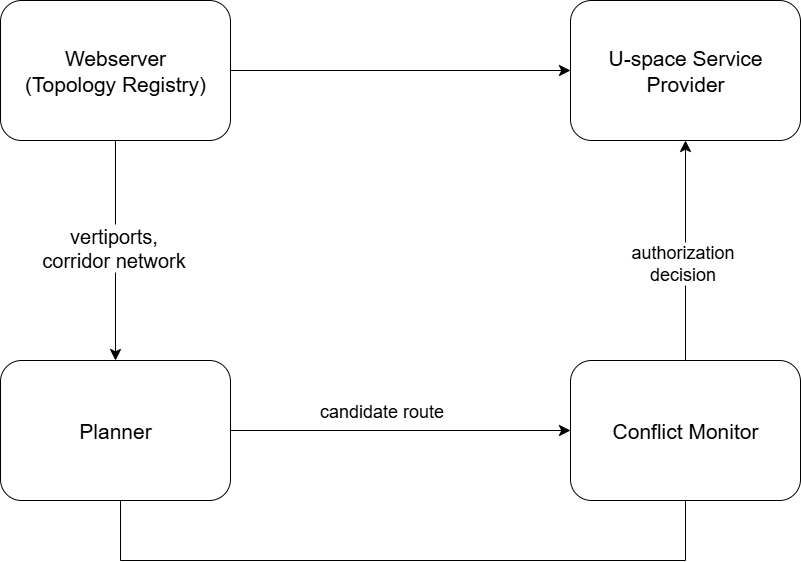
\includegraphics[width=0.5\textwidth]{figures/architecture.png}
  \caption{High-level architecture of the full-stack design. In the present implementation, the conflict-checking logic is embedded in the Planner.}
  \label{fig:architecture}
\end{figure}
